\documentclass[12pt,a4paper]{article}

% Packages
\usepackage[utf8]{inputenc}
\usepackage[T1]{fontenc}
\usepackage[english]{babel}
\usepackage{graphicx}
\usepackage{listings}
\usepackage{xcolor}
\usepackage{hyperref}
\usepackage{geometry}
\usepackage{fancyhdr}
\usepackage{titlesec}
\usepackage{float}
\usepackage{caption}
\usepackage{subcaption}
\usepackage{parskip}
\usepackage{microtype}

% Page geometry
\geometry{margin=2.5cm, headheight=15pt}

% Colors for code
\definecolor{codegreen}{rgb}{0,0.6,0}
\definecolor{codegray}{rgb}{0.5,0.5,0.5}
\definecolor{codepurple}{rgb}{0.58,0,0.82}
\definecolor{codeblue}{rgb}{0.13,0.29,0.53}
\definecolor{codeorange}{rgb}{0.8,0.4,0}
\definecolor{backcolour}{rgb}{0.97,0.97,0.97}
\definecolor{framecolor}{rgb}{0.8,0.8,0.8}

% Define JavaScript language for listings (used for TypeScript)
\lstdefinelanguage{JavaScript}{
  keywords={break, case, catch, continue, debugger, default, delete, do, else, finally, for, function, if, in, instanceof, new, return, switch, this, throw, try, typeof, var, void, while, with, let, const, class, export, extends, import, super, implements, interface, package, private, protected, public, static, yield, async, await, of, from, as, get, set, type, readonly, enum, abstract, declare, module, namespace, require},
  sensitive=true,
  comment=[l]{//},
  morecomment=[s]{/*}{*/},
  morestring=[b]',
  morestring=[b]",
  morestring=[b]`
}

% Define CSS language for listings
\lstdefinelanguage{CSS}{
  keywords={color, background, background-color, margin, padding, font, font-size, font-weight, border, border-radius, width, height, display, position, top, left, right, bottom, flex, grid, transition, transform, opacity, z-index, overflow, text-align, line-height, box-shadow, content, cursor, visibility, list-style, text-decoration, vertical-align, white-space, word-wrap, min-width, max-width, min-height, max-height, justify-content, align-items, flex-direction, flex-wrap, gap, var, hsl, rgb, rgba},
  sensitive=true,
  morecomment=[l]{//},
  morecomment=[s]{/*}{*/},
  morestring=[b]',
  morestring=[b]"
}

% Code listing style
\lstdefinestyle{mystyle}{
    backgroundcolor=\color{backcolour},
    commentstyle=\itshape\color{codegreen},
    keywordstyle=\bfseries\color{codeblue},
    numberstyle=\scriptsize\color{codegray},
    stringstyle=\color{codeorange},
    basicstyle=\ttfamily\small,
    breakatwhitespace=false,
    breaklines=true,
    captionpos=b,
    keepspaces=true,
    numbers=left,
    numbersep=8pt,
    showspaces=false,
    showstringspaces=false,
    showtabs=false,
    tabsize=2,
    frame=single,
    framerule=0.5pt,
    rulecolor=\color{framecolor},
    xleftmargin=15pt,
    framexleftmargin=15pt,
    aboveskip=12pt,
    belowskip=8pt,
    abovecaptionskip=8pt
}
\lstset{style=mystyle}

% Header and footer
\pagestyle{fancy}
\fancyhf{}
\fancyhead[L]{\small\textit{Distributed Systems Lab}}
\fancyhead[R]{\small\textit{Microservices Architecture}}
\fancyfoot[C]{\thepage}
\renewcommand{\headrulewidth}{0.4pt}
\renewcommand{\footrulewidth}{0.4pt}

% Title formatting
\titleformat{\section}{\Large\bfseries\color{codeblue}}{\thesection}{1em}{}[\vspace{0.5em}\hrule\vspace{0.5em}]
\titleformat{\subsection}{\large\bfseries}{\thesubsection}{1em}{}
\titleformat{\subsubsection}{\normalsize\bfseries}{\thesubsubsection}{1em}{}

% Hyperref setup
\hypersetup{
    colorlinks=true,
    linkcolor=codeblue,
    filecolor=magenta,
    urlcolor=codeblue,
    citecolor=codeblue,
    pdftitle={Microservices Architecture with Spring Cloud and Angular},
    pdfauthor={Otmane OUHAMI}
}

% Allow URL breaking
\makeatletter
\g@addto@macro{\UrlBreaks}{\UrlOrds}
\makeatother

% Fix overfull hboxes
\sloppy

\begin{document}

% ============================================
% TITLE PAGE
% ============================================
\begin{titlepage}
    \centering
    \vspace*{1cm}
    
    {\Large\textsc{ENSET Mohammedia}}\\[0.3cm]
    {\large\textsc{Hassan II University of Casablanca}}\\[0.5cm]
    {\large Master's Program in Software Engineering}\\[2cm]
    
    \rule{\textwidth}{1.5pt}\\[0.5cm]
    {\Huge\bfseries Microservices Architecture\\[0.3cm] with Spring Cloud and Angular}\\[0.5cm]
    \rule{\textwidth}{1.5pt}\\[1.5cm]
    
    {\Large\textsc{Distributed and Parallel Systems Laboratory}}\\[3cm]
    
    \begin{minipage}{0.5\textwidth}
        \begin{flushleft}
            \large\textbf{Prepared by:}\\[0.3cm]
            \Large Otmane OUHAMI
        \end{flushleft}
    \end{minipage}
    \hfill
    \begin{minipage}{0.4\textwidth}
        \begin{flushright}
            \large\textbf{Academic Year:}\\[0.3cm]
            \Large 2024 -- 2025
        \end{flushright}
    \end{minipage}
    
    \vfill
    
    {\large December 2024}
    
\end{titlepage}

% ============================================
% ABSTRACT PAGE
% ============================================
\newpage
\thispagestyle{empty}
\vspace*{3cm}
\begin{center}
    {\Large\bfseries Abstract}
\end{center}
\vspace{1cm}

\noindent
This report presents a comprehensive study and implementation of a microservices-based application using Spring Boot and Spring Cloud technologies. The project demonstrates the practical application of distributed systems concepts including service discovery, centralized configuration management, API gateway patterns, and inter-service communication.

\vspace{0.5cm}
\noindent
The system consists of multiple independent services working together to provide a cohesive billing and inventory management solution, complemented by a modern Angular frontend that interacts with the backend through a unified API gateway.

\vspace{0.5cm}
\noindent
Key technologies explored include Netflix Eureka for service discovery, Spring Cloud Config for centralized configuration, Spring Cloud Gateway for API routing, and OpenFeign for declarative REST clients. The frontend leverages Angular 19 with its modern signals-based reactive architecture.

\vspace{2cm}
\noindent\textbf{Keywords:} Microservices, Spring Boot, Spring Cloud, Angular, Service Discovery, API Gateway, Distributed Systems

% ============================================
% TABLE OF CONTENTS
% ============================================
\newpage
\tableofcontents
\newpage

% ============================================
\section{Introduction}
% ============================================

The evolution of software architecture has led to the widespread adoption of microservices as a preferred approach for building complex, scalable applications. Unlike monolithic architectures where all functionality resides within a single deployable unit, microservices decompose applications into small, independently deployable services that communicate over well-defined APIs.

This laboratory project explores the practical implementation of a microservices ecosystem using the Spring Cloud framework, which provides essential tools and patterns for building distributed systems. The application simulates a simplified e-commerce scenario with customer management, product inventory tracking, and billing functionalities, each implemented as separate microservices.

The primary objectives of this project include understanding service discovery mechanisms and their role in dynamic service location, implementing centralized configuration management for consistent application settings across services, utilizing an API gateway for request routing and load balancing, establishing inter-service communication using declarative REST clients, and developing a responsive frontend application using Angular with modern design patterns.

Through this implementation, we gain practical experience with the challenges and solutions inherent in distributed computing, including network latency, partial failures, and data consistency across service boundaries.

% ============================================
\section{System Architecture}
% ============================================

The architecture of this application follows the microservices pattern with several supporting infrastructure components that facilitate service coordination and communication. Understanding this architecture is fundamental to appreciating how the individual components work together as a cohesive system.

\subsection{Architecture Overview}

The system comprises six distinct services organized into two categories: infrastructure services that provide supporting functionality, and business services that implement the core application logic.

\begin{figure}[H]
    \centering
    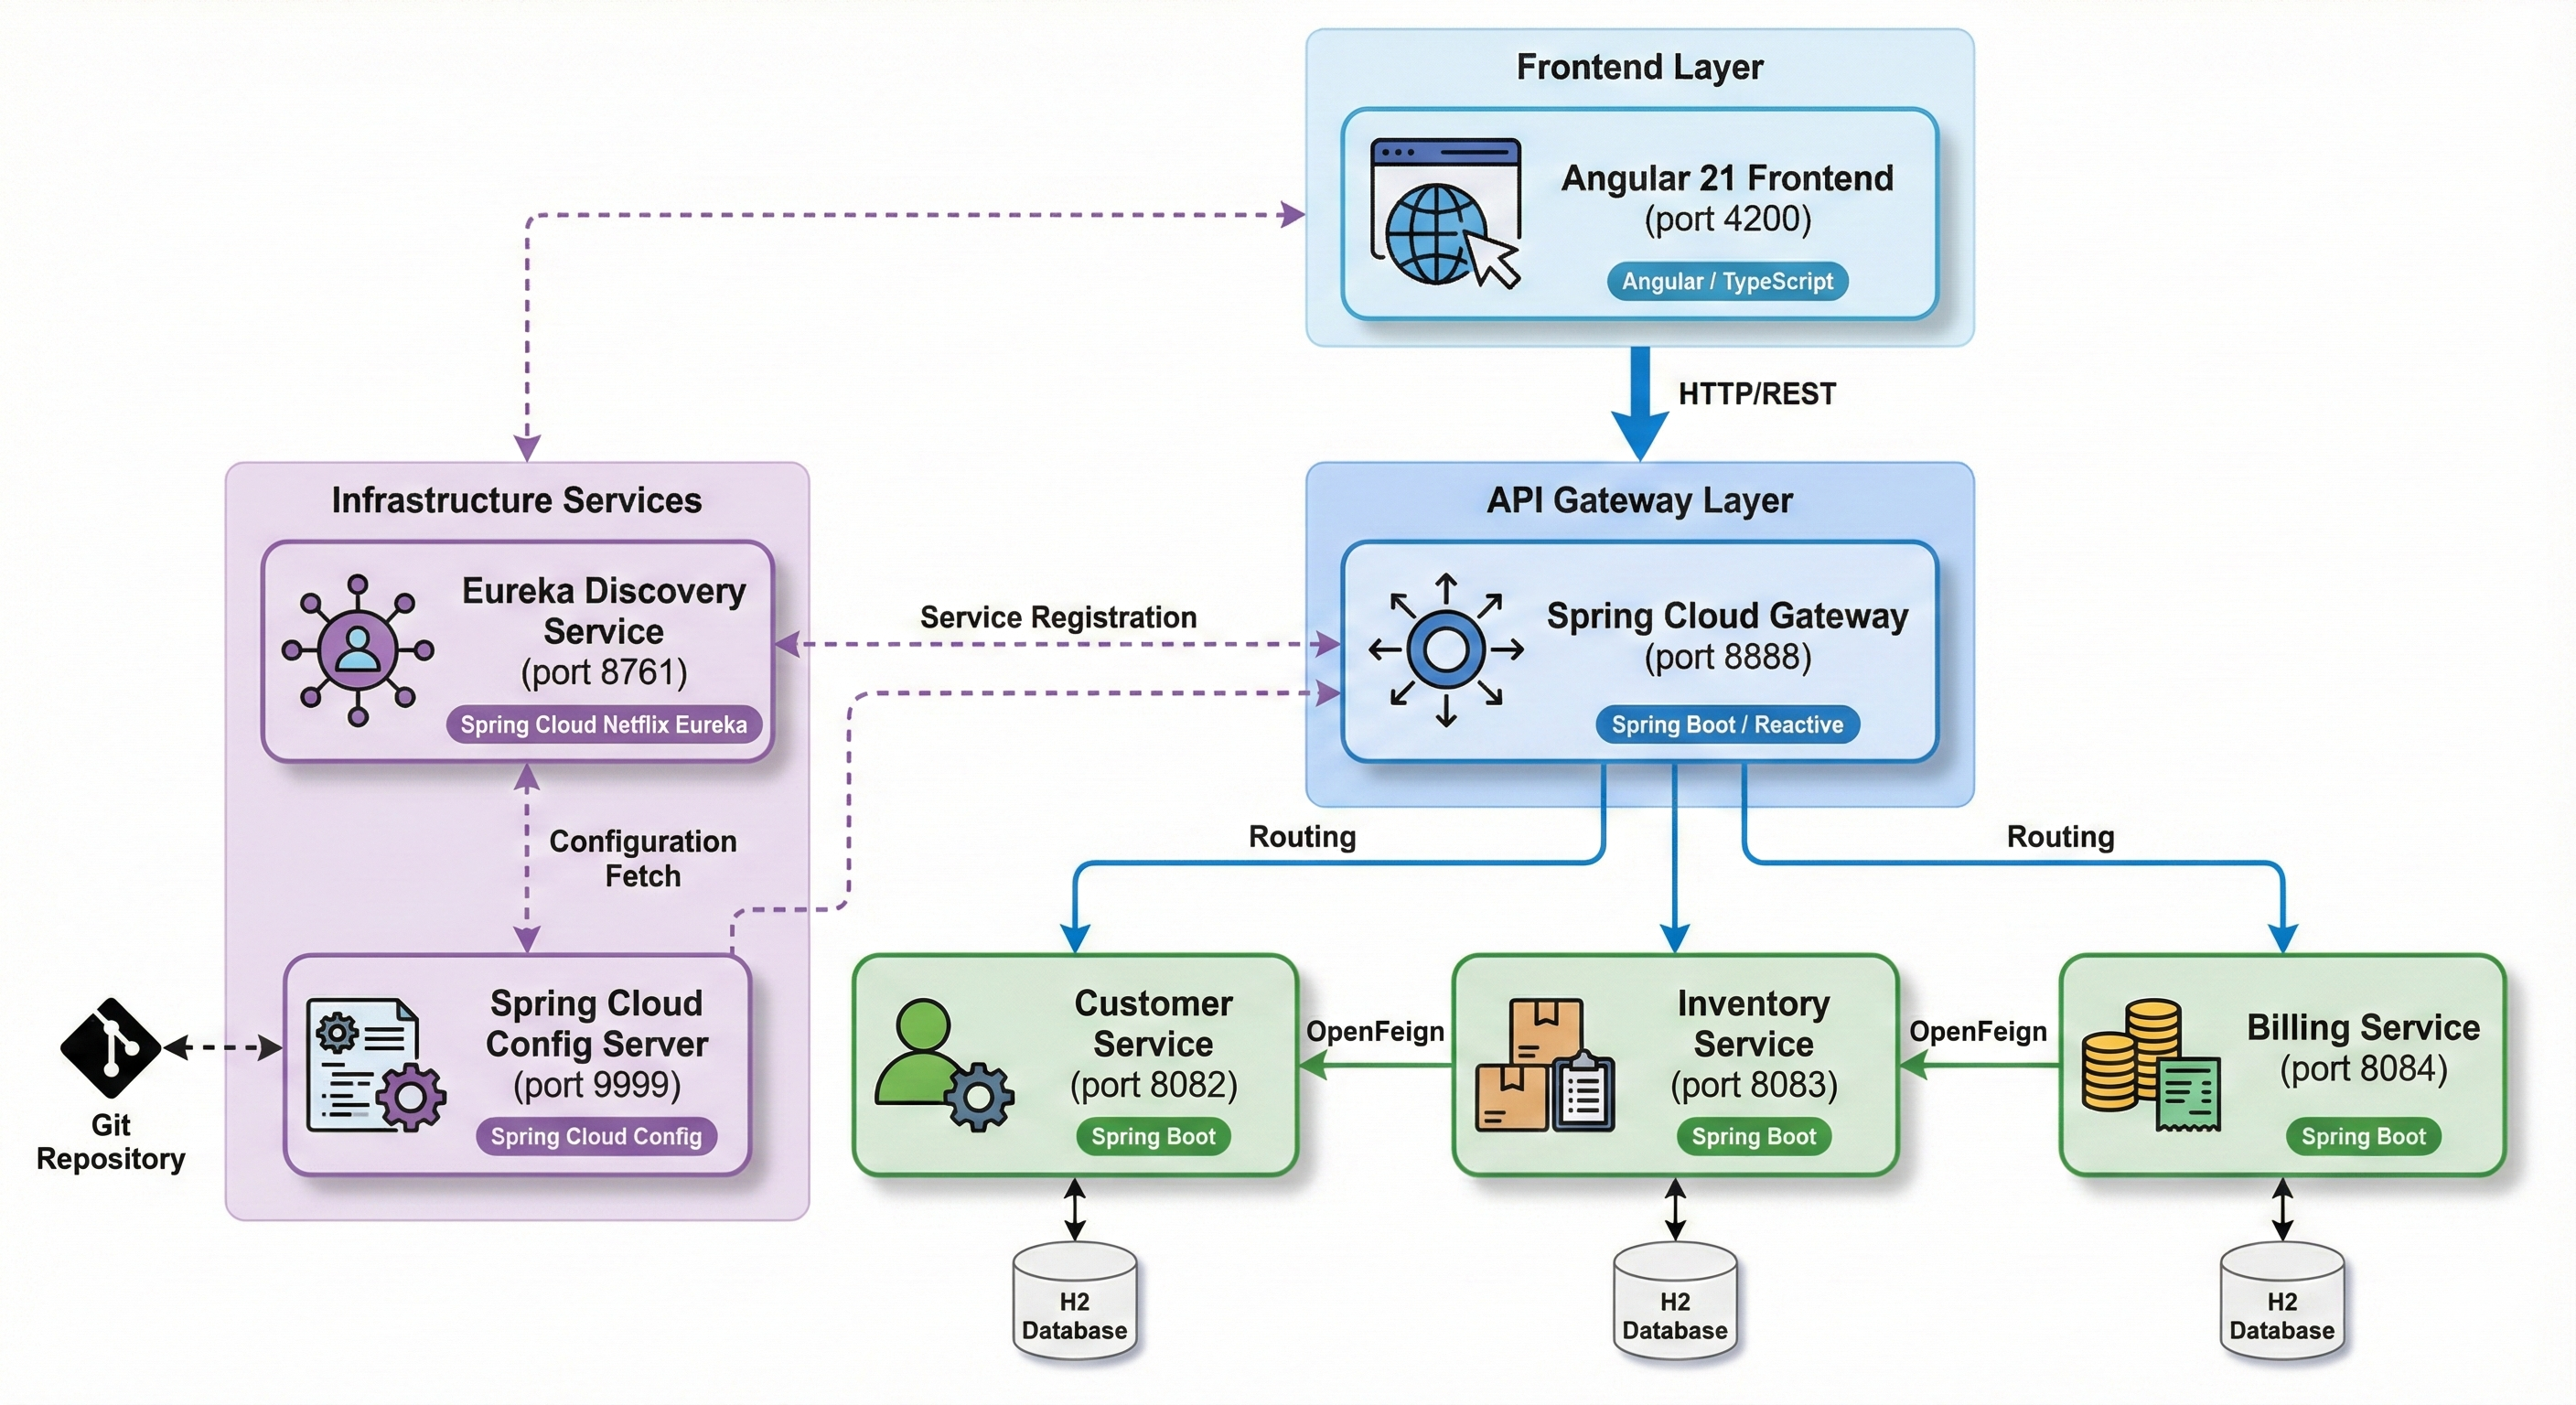
\includegraphics[width=\textwidth]{../screenshots/app-architecture.png}
    \caption{Complete microservices architecture showing all components and their interactions}
    \label{fig:architecture}
\end{figure}

As illustrated in Figure \ref{fig:architecture}, the architecture demonstrates several key patterns. The Discovery Service acts as a service registry where all microservices register themselves upon startup. The Config Service provides externalized configuration, allowing services to retrieve their settings from a centralized Git repository. The Gateway Service serves as the single entry point for all client requests, routing them to appropriate backend services. The three business services, namely Customer Service, Inventory Service, and Billing Service, each maintain their own database and expose REST APIs for their respective domains.

\subsection{Technology Stack}

The implementation leverages a carefully selected technology stack that provides robust support for microservices development. The backend is built entirely with Spring Boot 3.5.6, utilizing Java 21 as the runtime environment. Spring Cloud 2025.0.0 provides the distributed systems infrastructure components. Each service uses Spring Data JPA with H2 in-memory databases for data persistence, while Spring Data REST automatically exposes repository methods as RESTful endpoints.

The frontend application is developed using Angular 19 with TypeScript, employing a signals-based reactive architecture for optimal performance. The styling follows a shadcn-inspired design system implemented in pure CSS, providing a modern and professional user interface.

\newpage
% ============================================
\section{Infrastructure Services}
% ============================================

Infrastructure services form the backbone of the microservices ecosystem, providing essential capabilities that enable the business services to function effectively in a distributed environment.

\subsection{Discovery Service with Netflix Eureka}

Service discovery is a fundamental requirement in microservices architectures where services need to locate and communicate with each other dynamically. Netflix Eureka, integrated through Spring Cloud Netflix, provides this capability by maintaining a registry of available service instances.

The Discovery Service is configured as an Eureka Server, as shown in the following Spring Boot application class:

\begin{lstlisting}[language=Java, caption=Discovery Service Main Application]
@SpringBootApplication
@EnableEurekaServer
public class DiscoveryServiceApplication {
    public static void main(String[] args) {
        SpringApplication.run(DiscoveryServiceApplication.class, args);
    }
}
\end{lstlisting}

The \texttt{@EnableEurekaServer} annotation transforms this Spring Boot application into a service registry. When other services start, they automatically register with this server and periodically send heartbeat signals to indicate their availability. If a service fails to send heartbeats, Eureka marks it as unavailable and eventually removes it from the registry.

The configuration for the Discovery Service specifies that it should not register itself or fetch the registry, as it is the registry itself:

\begin{lstlisting}[caption=Discovery Service Configuration]
server.port=8761
spring.application.name=discovery-service
eureka.client.register-with-eureka=false
eureka.client.fetch-registry=false
\end{lstlisting}

\subsection{Config Service with Spring Cloud Config}

Managing configuration across multiple services presents significant challenges, particularly when configurations need to change without redeploying services. Spring Cloud Config addresses this by providing a centralized configuration server that serves configuration properties from a Git repository.

\begin{lstlisting}[language=Java, caption=Config Service Main Application]
@SpringBootApplication
@EnableConfigServer
public class ConfigServiceApplication {
    public static void main(String[] args) {
        SpringApplication.run(ConfigServiceApplication.class, args);
    }
}
\end{lstlisting}

The configuration server connects to a Git repository containing property files for each service. When a service requests its configuration, the Config Server retrieves the appropriate file based on the service name and active profiles.

\begin{lstlisting}[caption=Config Service Properties]
server.port=9999
spring.application.name=config-service
spring.cloud.config.server.git.uri=file:///path/to/config-repo
\end{lstlisting}

This approach enables configuration changes without service redeployment, version control for configuration history, environment-specific configurations through profile support, and consistent configuration management across all services.

\subsection{Gateway Service with Spring Cloud Gateway}

The API Gateway pattern provides a single entry point for all client requests, offering benefits such as request routing, protocol translation, and cross-cutting concerns like authentication and rate limiting. Spring Cloud Gateway implements this pattern using a reactive, non-blocking architecture built on Project Reactor.

\begin{lstlisting}[language=Java, caption=Gateway Service Configuration]
@SpringBootApplication
public class GatewayServiceApplication {
    public static void main(String[] args) {
        SpringApplication.run(GatewayServiceApplication.class, args);
    }

    @Bean
    DiscoveryClientRouteDefinitionLocator routeDefinitionLocator(
            ReactiveDiscoveryClient discoveryClient,
            DiscoveryLocatorProperties properties) {
        return new DiscoveryClientRouteDefinitionLocator(
            discoveryClient, properties);
    }
}
\end{lstlisting}

The \texttt{DiscoveryClientRouteDefinitionLocator} bean enables dynamic route discovery. Rather than manually configuring routes for each service, the gateway automatically creates routes based on services registered with Eureka. When a request arrives at \texttt{/customer-service/api/customers}, the gateway resolves the customer-service through Eureka and forwards the request to an available instance.

Cross-Origin Resource Sharing (CORS) configuration is essential when the frontend application runs on a different origin than the backend services:

\begin{lstlisting}[language=Java, caption=CORS Configuration for Gateway]
@Configuration
public class CorsConfig {
    @Bean
    public CorsWebFilter corsWebFilter() {
        CorsConfiguration corsConfig = new CorsConfiguration();
        corsConfig.setAllowedOrigins(List.of("http://localhost:4200"));
        corsConfig.setAllowedMethods(Arrays.asList(
            "GET", "POST", "PUT", "DELETE", "PATCH", "OPTIONS"));
        corsConfig.setAllowedHeaders(List.of("*"));
        corsConfig.setAllowCredentials(true);
        
        UrlBasedCorsConfigurationSource source = 
            new UrlBasedCorsConfigurationSource();
        source.registerCorsConfiguration("/**", corsConfig);
        return new CorsWebFilter(source);
    }
}
\end{lstlisting}

\newpage
% ============================================
\section{Business Services}
% ============================================

The business services implement the core functionality of the application, each responsible for a specific domain within the system. Following the microservices principle of single responsibility, each service manages its own data and exposes a well-defined API.

\subsection{Customer Service}

The Customer Service manages customer information, providing operations for creating, reading, updating, and deleting customer records. The service uses Spring Data REST to automatically expose repository methods as RESTful endpoints.

\begin{lstlisting}[language=Java, caption=Customer Entity Definition]
@Entity
@NoArgsConstructor
@AllArgsConstructor
@Getter @Setter @Builder
public class Customer {
    @Id
    @GeneratedValue(strategy = GenerationType.IDENTITY)
    private Long id;
    private String name;
    private String email;
}
\end{lstlisting}

The repository interface extends \texttt{JpaRepository} and is annotated with \texttt{@RepositoryRestResource}, which instructs Spring Data REST to expose CRUD operations automatically:

\begin{lstlisting}[language=Java, caption=Customer Repository with REST Exposure]
@RepositoryRestResource
public interface CustomerRepository 
        extends JpaRepository<Customer, Long> {
}
\end{lstlisting}

This minimal configuration generates a complete REST API with endpoints for listing all customers, retrieving individual customers by ID, creating new customers, updating existing customers, and deleting customers. The API follows HATEOAS principles, including hypermedia links in responses for discoverability.

\subsection{Inventory Service}

The Inventory Service manages the product catalog and stock levels. Products are identified by UUID to ensure globally unique identifiers across distributed systems.

\begin{lstlisting}[language=Java, caption=Product Entity with UUID Identifier]
@Entity
@NoArgsConstructor
@AllArgsConstructor
@Getter @Setter @Builder
public class Product {
    @Id
    @GeneratedValue(strategy = GenerationType.UUID)
    private UUID id;
    private String name;
    private double price;
    private int quantity;
}
\end{lstlisting}

Beyond the standard CRUD operations provided by Spring Data REST, the Inventory Service exposes additional endpoints for inventory management operations such as updating stock quantities:

\begin{lstlisting}[language=Java, caption=Inventory Controller for Stock Management]
@RestController
@RequestMapping("/inventory")
@RequiredArgsConstructor
public class ProductRestController {
    private final ProductRepository productRepository;

    @PostMapping("/products/{id}/update-quantity")
    public ResponseEntity<Product> updateQuantity(
            @PathVariable UUID id,
            @RequestParam int delta) {
        return productRepository.findById(id)
            .map(product -> {
                int newQuantity = product.getQuantity() + delta;
                if (newQuantity < 0) {
                    return ResponseEntity.badRequest().<Product>build();
                }
                product.setQuantity(newQuantity);
                return ResponseEntity.ok(productRepository.save(product));
            })
            .orElse(ResponseEntity.notFound().build());
    }
}
\end{lstlisting}

\subsection{Billing Service}

The Billing Service represents the most complex component, managing bills and their associated line items. This service demonstrates inter-service communication by fetching customer and product details from other services.

\begin{lstlisting}[language=Java, caption=Bill Entity with Relationships]
@Entity
@NoArgsConstructor
@AllArgsConstructor
@Getter @Setter @Builder
public class Bill {
    @Id
    @GeneratedValue(strategy = GenerationType.IDENTITY)
    private Long id;
    private Date billingDate;
    private Long customerId;
    
    @OneToMany(mappedBy = "bill")
    private List<ProductItem> productItems = new ArrayList<>();
    
    @Transient
    private Customer customer;
}
\end{lstlisting}

The \texttt{@Transient} annotation on the customer field indicates that this property is not persisted in the database. Instead, it is populated at runtime by fetching data from the Customer Service.

\subsection{Inter-Service Communication with OpenFeign}

OpenFeign provides a declarative approach to building REST clients. Rather than manually constructing HTTP requests, developers define interfaces annotated with Spring MVC annotations, and Feign generates the implementation.

\begin{lstlisting}[language=Java, caption=Feign Client for Customer Service]
@FeignClient(name = "customer-service")
public interface CustomerRestClient {
    @GetMapping("/api/customers/{id}")
    Customer getCustomerById(@PathVariable("id") Long id);

    @GetMapping("/api/customers")
    PagedModel<Customer> getCustomers();
}
\end{lstlisting}

The \texttt{name} attribute specifies the service name as registered in Eureka. Feign integrates with the service discovery mechanism to resolve the actual service location at runtime. This abstraction means that the calling code does not need to know the physical address of the target service.

The Billing Service uses these Feign clients to enrich bill data with customer and product information:

\begin{lstlisting}[language=Java, caption=Bill Controller with Service Integration]
@RestController
@RequiredArgsConstructor
public class BillRestController {
    private final BillRepository billRepository;
    private final ProductItemRepository productItemRepository;
    private final CustomerRestClient customerRestClient;
    private final ProductRestClient productRestClient;

    @GetMapping("/bills/full/{id}")
    public Bill getBill(@PathVariable Long id) {
        Bill bill = billRepository.findById(id)
            .orElseThrow(() -> new RuntimeException("Bill not found"));
        
        bill.setCustomer(customerRestClient.getCustomerById(
            bill.getCustomerId()));
        
        bill.getProductItems().forEach(item -> {
            item.setProduct(productRestClient.getProductById(
                item.getProductId()));
        });
        
        return bill;
    }
}
\end{lstlisting}

\newpage
% ============================================
\section{Frontend Application}
% ============================================

The frontend provides a user-friendly interface for interacting with the microservices backend. Built with Angular 19, it employs modern development practices including standalone components, signals for reactive state management, and a custom CSS design system inspired by shadcn/ui.

\subsection{Application Structure}

The Angular application follows a modular structure that promotes maintainability and scalability. Services encapsulate HTTP communication logic, while components manage presentation and user interaction.

\begin{lstlisting}[language=JavaScript, caption=Customer Service in Angular (TypeScript)]
@Injectable({ providedIn: 'root' })
export class CustomerService {
  private http = inject(HttpClient);
  private baseUrl = `${environment.apiBaseUrl}/customer-service/api/customers`;

  getAll(): Observable<Customer[]> {
    return this.http.get<PagedResponse<Customer>>(this.baseUrl).pipe(
      map(response => response._embedded?.customers || [])
    );
  }

  create(customer: Customer): Observable<Customer> {
    return this.http.post<Customer>(this.baseUrl, customer);
  }

  update(id: number, customer: Customer): Observable<Customer> {
    return this.http.put<Customer>(`${this.baseUrl}/${id}`, customer);
  }

  delete(id: number): Observable<void> {
    return this.http.delete<void>(`${this.baseUrl}/${id}`);
  }
}
\end{lstlisting}

All HTTP requests are routed through the API Gateway at port 8888, which forwards them to the appropriate backend service. This approach provides a single point of entry, simplifying CORS configuration and enabling future enhancements such as authentication middleware.

\subsection{Reactive State Management with Signals}

Angular signals provide a reactive primitive for managing component state. Unlike the traditional change detection approach that relies on Zone.js, signals explicitly track dependencies and update only the affected parts of the view.

\begin{lstlisting}[language=JavaScript, caption=Component Using Signals (TypeScript)]
@Component({
  selector: 'app-customers',
  standalone: true,
  imports: [CommonModule, FormsModule],
  templateUrl: './customers.component.html'
})
export class CustomersComponent implements OnInit {
  private customerService = inject(CustomerService);

  customers = signal<Customer[]>([]);
  loading = signal(true);
  showModal = signal(false);

  loadCustomers() {
    this.loading.set(true);
    this.customerService.getAll().subscribe({
      next: (data) => {
        this.customers.set(data);
        this.loading.set(false);
      },
      error: (err) => {
        console.error('Error loading customers:', err);
        this.loading.set(false);
      }
    });
  }
}
\end{lstlisting}

This approach eliminates the need for Zone.js and provides more predictable change detection behavior, improving application performance.

\subsection{Design System and Styling}

The application employs a custom CSS design system that provides consistent styling across all components. Using CSS custom properties enables easy theming and maintains visual consistency.

\begin{lstlisting}[language=CSS, caption=CSS Design System Variables]
:root {
  --background: 0 0% 100%;
  --foreground: 240 10% 3.9%;
  --primary: 240 5.9% 10%;
  --primary-foreground: 0 0% 98%;
  --muted: 240 4.8% 95.9%;
  --border: 240 5.9% 90%;
  --radius: 0.5rem;
}

.btn-primary {
  background: hsl(var(--primary));
  color: hsl(var(--primary-foreground));
  padding: 0.5rem 1rem;
  border-radius: var(--radius);
  transition: opacity 0.2s;
}
\end{lstlisting}

\subsection{User Interface}

The frontend provides intuitive interfaces for managing customers, products, and bills. Each view includes data tables with action buttons, modal forms for creating and editing records, and visual feedback for loading states.

\begin{figure}[H]
    \centering
    \includegraphics[width=0.9\textwidth]{../screenshots/customers-ui.png}
    \caption{Customer management interface displaying the list of customers with action buttons}
    \label{fig:customers-ui}
\end{figure}

The customer management interface shown in Figure \ref{fig:customers-ui} presents customers in a clean table format with options to edit or delete each record. The interface follows accessibility best practices with clear labels and consistent interaction patterns.

\begin{figure}[H]
    \centering
    \includegraphics[width=0.9\textwidth]{../screenshots/add-customer-ui.png}
    \caption{Modal dialog for adding a new customer}
    \label{fig:add-customer}
\end{figure}

\begin{figure}[H]
    \centering
    \includegraphics[width=0.9\textwidth]{../screenshots/products-ui.png}
    \caption{Product inventory interface showing stock levels and product details}
    \label{fig:products-ui}
\end{figure}

The product management interface in Figure \ref{fig:products-ui} displays the inventory with stock status indicators. Products with sufficient stock are marked as "In Stock" while those with low quantities receive appropriate visual warnings.

\begin{figure}[H]
    \centering
    \includegraphics[width=0.9\textwidth]{../screenshots/edit-product-ui.png}
    \caption{Product editing form with price and quantity fields}
    \label{fig:edit-product}
\end{figure}

\begin{figure}[H]
    \centering
    \includegraphics[width=0.9\textwidth]{../screenshots/bills-ui.png}
    \caption{Bills listing interface showing all invoices}
    \label{fig:bills-ui}
\end{figure}

The billing interface in Figure \ref{fig:bills-ui} presents all invoices with their associated customers. Users can view detailed bill information including individual line items and their totals.

\begin{figure}[H]
    \centering
    \includegraphics[width=0.9\textwidth]{../screenshots/manage-bill-ui.png}
    \caption{Detailed bill view with product items and total calculation}
    \label{fig:manage-bill}
\end{figure}

Figure \ref{fig:manage-bill} shows the bill detail view where users can see all items included in a bill, their quantities, unit prices, and the computed total. This view also allows adding new items to an existing bill or removing items, with automatic inventory updates.

\newpage
% ============================================
\section{API Documentation with OpenAPI}
% ============================================

The project integrates SpringDoc OpenAPI to provide interactive API documentation. Each service exposes its API specification through Swagger UI, accessible at the \texttt{/swagger-ui.html} endpoint.

The Gateway Service aggregates documentation from all downstream services, providing a unified view of the entire API surface. This configuration is achieved through a dedicated SwaggerConfig class that registers each service's documentation endpoint:

\begin{lstlisting}[language=Java, caption=Swagger Aggregation Configuration]
@Configuration
public class SwaggerConfig {
    @Bean
    @Lazy(false)
    public Set<SwaggerUrl> swaggerUrls(
            RouteDefinitionLocator locator,
            SwaggerUiConfigProperties swaggerUiConfigProperties) {
        Set<SwaggerUrl> urls = new HashSet<>();
        
        List<String> services = List.of(
            "customer-service",
            "inventory-service",
            "billing-service"
        );
        
        services.forEach(service -> {
            SwaggerUrl swaggerUrl = new SwaggerUrl();
            swaggerUrl.setName(service);
            swaggerUrl.setUrl("/" + service + "/v3/api-docs");
            urls.add(swaggerUrl);
        });
        
        swaggerUiConfigProperties.setUrls(urls);
        return urls;
    }
}
\end{lstlisting}

Accessing the Gateway's Swagger UI at \texttt{http://localhost:8888/swagger-ui.html} presents a dropdown menu allowing users to select and explore the documentation for each individual service.

\newpage
% ============================================
\section{Conclusion}
% ============================================

This project has provided valuable hands-on experience with microservices architecture using Spring Cloud and Angular. Through the implementation of a complete distributed system, we have explored key concepts and patterns that are essential in modern software development.

The service discovery pattern, implemented using Netflix Eureka, demonstrated how services can dynamically locate each other without hardcoded addresses. This capability is fundamental in cloud environments where service instances may scale up or down and their addresses may change frequently. The centralized configuration approach with Spring Cloud Config showed how application settings can be managed consistently across all services, enabling configuration changes without redeployment.

The API Gateway pattern proved invaluable for simplifying client communication with the backend services. By providing a single entry point, the gateway eliminated the need for clients to know the locations of individual services and enabled centralized handling of cross-cutting concerns such as CORS. The inter-service communication through OpenFeign demonstrated how microservices can collaborate while remaining loosely coupled, with the billing service fetching data from customer and inventory services transparently.

On the frontend, Angular's modern features including standalone components and signals provided an efficient approach to building reactive user interfaces. The separation of concerns between services, components, and styling facilitated maintainable code organization, while the custom CSS design system ensured visual consistency throughout the application.

Looking forward, this architecture could be extended with additional capabilities such as distributed tracing for debugging request flows across services, circuit breakers for improved resilience against service failures, message queues for asynchronous communication, and containerization with Docker and Kubernetes for deployment. The solid foundation established in this project provides a starting point for exploring these advanced topics in distributed systems.

The experience gained through this implementation reinforces the importance of understanding distributed systems fundamentals. While microservices offer significant benefits in terms of scalability and team autonomy, they also introduce complexity that must be carefully managed through proper architectural patterns and infrastructure components.

\end{document}
